\graphicspath{{4int/asy/}}

\section{Integration}

The theory of infinite series addresses how to sum infinitely many \emph{finite} quantities. Integration, by contrast, is the business of summing infinitely many \emph{infinitesimal} quantities. Attempts to do both have been part of mathematics for well over 2000 years, and the philosophical objections are just as old.\footnote{%
	Two of Zeno's ancient paradoxes are relevant here: Achilles and the Tortoise concerns a convergent infinite series, while the Arrow Paradox toys with integration by questioning whether time can be viewed as a sum of instants. Perhaps the most famous contemporary criticism comes from Bishop George Berkeley, who gave his name to the city and first UC campus: in 1734's \href{https://en.wikipedia.org/wiki/The_Analyst}{\emph{The Analyst}}, Berkeley savaged the foundations of calculus, describing the infinitesimal increments required in Newton's theory of \emph{fluxions} (derivatives) as merely the ``ghosts of departed quantities.''%
} The development and increased application of calculus from the late 1600s onward spurred mathematicians to put the theory on a firmer footing, though from Newton and Leibniz it took another 150 years before Bernhard Riemann (1856) provided a thorough development of the integral.



\setcounter{subsection}{31}
\subsection{The Riemann Integral}\label{sec:riemann}

The basic idea behind Riemann integration is to approximate area using a sequence of rectangles whose \emph{width} tends to zero. The following discussion illustrates the essential idea, which should be familiar from elementary calculus.

\begin{example}[lower separated=false, sidebyside, sidebyside align=top seam, sidebyside gap=0pt, righthand width=0.37\linewidth]{}{riemannintro}
	Suppose $f(x)=x^2$ is defined on $[0,1]$.\medbreak
	For each $n\in\N$, let $\Delta x=\frac 1n$ and define $x_i=i\Delta x$.\smallbreak
	Above each \emph{subinterval} $[x_{i-1},x_i]$, raise a rectangle of height $f(x_i)=x_i^2$. The sum of the areas of these rectangles is the \emph{Riemann sum with right-endpoints}\footnotemark
	\begin{align*}
	  R_n&=\sum_{i=1}^n f(x_i)\Delta x 
	  =\sum_{i=1}^n\frac{i^2}{n^3}
	  =\frac{n(n+1)(2n+1)}{6n^3}\\ 
	  &=\frac 13+\frac{3n+1}{6n^2}
	\end{align*}
	
	The \emph{Riemann sum with left-endpoints} is defined similarly:
	\begin{align*}
	  L_n&=\sum_{i=1}^n f(x_{i-1})\Delta x 
	  =\sum_{i=1}^n\frac{(i-1)^2}{n^3} =\frac 13-\frac{3n-1}{6n^2}
	\end{align*}
	Since $f$ is an increasing function, the area $A$ under the curve plainly satisfies
	\[
		L_n\le A\le R_n
	\]
	By the squeeze theorem, we conclude that $A=\frac 13$.
	\tcblower
	\vspace{-5pt}
	\flushright\href{https://www.math.uci.edu/~ndonalds/math140b/riemann.html}{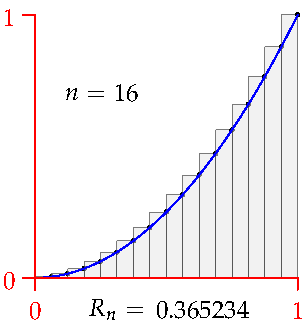
\includegraphics[scale=0.95]{area-up}\smallbreak
	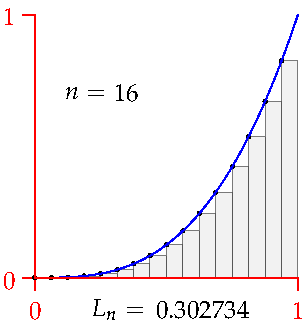
\includegraphics[scale=0.95]{area-down}}
\end{example}

The example should feel convincing, though perhaps this is due to the simplicity of the function. To apply this approach to more general functions, we need to be significantly more rigorous.

\footnotetext{%
	Recall some basic identities:
	$\sum\limits_{i=1}^n i=\frac 12n(n+1)$, \ $\sum\limits_{i=1}^n i^2=\frac 16n(n+1)(2n+1)$, \ $\sum\limits_{i=1}^n i^3=\frac 14n^2(n+1)^2$%
}


\goodbreak


\begin{defn}{}{}
	A \emph{partition} $P=\{x_0,\ldots,x_n\}$ of an interval $[a,b]$ is a finite sequence for which
	\[
		a=x_0<x_1<\cdots< x_{n-1}< x_n=b
	\]
	Choosing a \emph{sample point} $x_i^*$ in each \emph{subinterval} $[x_{i-1},x_i]$ results in a \emph{tagged partition}.\smallbreak
	The \emph{mesh} of the partition is $\mesh(P):=\max\Delta x_i$, the width $\Delta x_i=x_i-x_{i-1}$ of the largest subinterval.\smallbreak
	If $f:[a,b]\to\R$, the \emph{Riemann sum} \smash{$\sum_{i=1}^n f(x_i^*)\,\Delta x_i$} evaluates the area of a family of $n$ rectangles, as pictured. The heights $f(x_i^*)$ and thus areas can be negative or zero.
	\begin{center}
	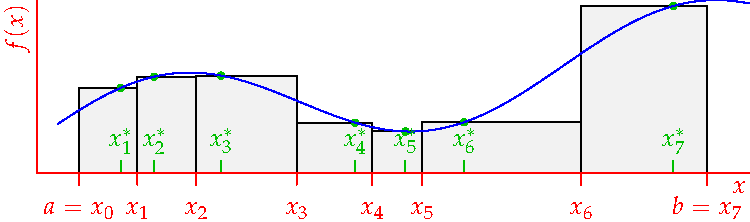
\includegraphics[scale=0.95]{riemann-sum}
	\end{center}
\end{defn}

In elementary calculus, one typically computes Riemann sums for \emph{equally-spaced} partitions with \emph{left,} \emph{right} or \emph{middle} sample points. The flexibility of tagged partitions makes applying Riemann's definition a challenge, so we instead consider two special families of rectangles. 


\begin{defn}{}{darbouxint}
	Given a partition $P$ of $[a,b]$ and a bounded function $f$ on $[a,b]$, define\par
	\begin{minipage}[t]{0.6\linewidth}\vspace{-15pt}
		\begin{align*}
			&M_i=\!\!\sup_{x\in [x_{i-1},x_i]}\! f(x)\qquad &&U(f,P)=\sum_{i=1}^n M_i\,\Delta x_i\\
			&m_i=\!\!\inf_{x\in [x_{i-1},x_i]}\! f(x) &&L(f,P)=\sum_{i=1}^n m_i\,\Delta x_i
		\end{align*}
		$U(f,P)$ and $L(f,P)$ are the \emph{upper} and \emph{lower Darboux sums} for $f$ with respect to $P$.
		The \emph{upper} and \emph{lower Darboux integrals} are
		% \begin{gather*}
		% U(f)=\upint_a^b f(x)\,\dx:=\inf\{U(f,P):P\text{ is a partition of $[a,b]$}\}\\
		% L(f)=\lowint_a^bf(x)\,\dx:=\sup\{L(f,P):P\text{ is a partition of $[a,b]$}\}
		% \end{gather*}
		\[
			U(f)=\inf U(f,P)\qquad L(f)=\sup L(f,P)
		\]
		where the supremum/infimum are taken over all partitions. Necessarily both integrals are \emph{finite.}\smallbreak
		We say that $f$ is \emph{(Riemann) integrable} on $[a,b]$ if $U(f)=L(f)$. We denote this value by
		\[
			\int_a^bf\quad\text{or}\quad\int_a^bf(x)\,\dx
		\]
		\end{minipage}
		\hfill
		\begin{minipage}[t]{0.39\linewidth}\vspace{-5pt}
			\centering
			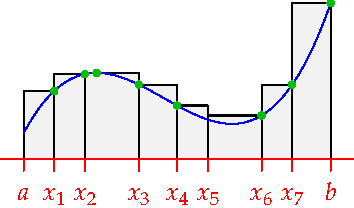
\includegraphics[scale=0.95]{darboux-sum-upper}\par
			Upper Darboux sum $U(f,P)$\bigbreak
			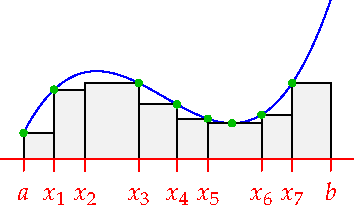
\includegraphics[scale=0.95]{darboux-sum-lower}\par
			Lower Darboux sum $L(f,P)$
		\end{minipage}\medbreak
	If the interval is understood or irrelevant, one often simply says that $f$ is integrable and writes $\int f$.
	% We say that $f$ is integrable on a bounded interval $(a,b)$ if every extension of $f$ to $[a,b]$ is integrable.\smallbreak
\end{defn}


Intuitively, $L(f,P)$ is the sum of the areas of rectangles built on $P$ which just fit under the graph of $f$. It is also the infimum of all Riemann sums on $P$. If $f$ is discontinuous, then $L(f,P)$ need not itself be a Riemann sum, as there might not exist suitable sample points!

\goodbreak

\begin{examples}{}{}
	\exstart We revisit Example \ref{ex:riemannintro} in this language.
	\begin{enumerate}\setcounter{enumi}{1}
	  \item[]Given a partition $Q=\{x_0,\ldots,x_n\}$ of $[0,1]$ and sample points $x_i^*\in[x_{i-1},x_i]$, we compute the Riemann sum for $f(x)=x^2$
		\[
			\sum_{i=1}^nf(x_i^*)\,\Delta x_i=\sum_{i=1}^n(x_i^*)^2(x_i-x_{i-1})
		\]
		Since $f$ is increasing,  we have $x_{i-1}^2\le (x_i^*)^2\le x_i^2$ on each interval, whence
		\[
			L(f,Q) =\sum_{i=1}^n(x_{i-1})^2(x_i-x_{i-1})
			\le\sum_{i=1}^n(x_i^*)^2(x_i-x_{i-1})
			\le\sum_{i=1}^n(x_i)^2(x_i-x_{i-1})=U(f,Q)
		\]
		The Darboux sums are therefore the Riemann sums for left- and right-endpoints.\smallbreak
		If we take $Q_n$ to be the partition with subintervals of equal width $\Delta x=\frac 1n$, then
		\[
			U(f)=\inf_P U(f,P)\le U(f,Q_n)
			=\sum_{i=1}^n\left(\frac in\right)^2\!\Delta x =R_n
		\]
		is the right Riemann sum discussed originally. Similarly $L(f)\ge L_n$. Since $L_n$ and $R_n$ both converge to $\frac 13$ as $n\to \infty$, the squeeze theorem forces
		\[
			L_n\le L(f)\le U(f)\le R_n
			\implies L(f)=U(f)=\frac 13
		\]
		Otherwise said, $f$ is integrable on $[0,1]$ with $\int_0^1x^2\,\dx=\frac 13$.

		\begin{minipage}[t]{0.58\linewidth}\vspace{0pt}
			\item Suppose $f(x)=kx+c$ on $[a,b]$, and that $k>0$. Take the evenly spaced partition $P_n$ where $x_i=a+\frac{b-a}ni$. Since $f$ is increasing, the upper Darboux sum is again the Riemann sum with right-endpoints:
			\begin{align*}
				U(f,P_n)
				&=R_n=\sum_{i=1}^nf(x_i)\Delta x\\
				&=\frac{b-a}n\sum_{i=1}^n\frac{k(b-a)}ni+ak+c
			\end{align*}
		\end{minipage}
		\hfill
		\begin{minipage}[t]{0.4\linewidth}\vspace{0pt}
			\flushright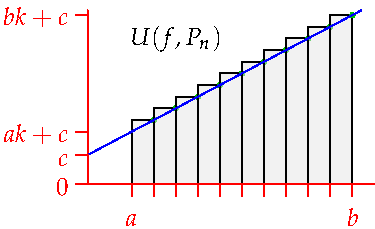
\includegraphics[scale=0.95]{darboux-triangle}
		\end{minipage}\vspace{-5pt}
  
		\begin{align*}
			\phantom{U(f,P_n)}
			&=\frac{b-a}n\left[\frac{k(b-a)}n\cdot \frac 12n(n+1)+(ak+c)n\right]\\
			&\xrightarrow[n\to\infty]{} \frac 12k(b-a)^2+(b-a)(ak+c)
				=\frac k2(b^2-a^2)+c(b-a)
		\end{align*}
		Similarly, the lower Darboux sum is the Riemann sum with left-endpoints:
		\[
			L(f,P_n)=L_n
			=\frac{b-a}n\left[\frac{k(b-a)}n\cdot \frac 12n(n-1)+(ak+c)n\right] 
			\xrightarrow[n\to\infty]{} \frac k2(b^2-a^2)+c(b-a)
		\]
		As above, $L_n\le L(f)\le U(f)\le R_n$ and the squeeze theorem prove that $f$ is integrable on $[a,b]$ with $\int_a^bf=\frac k2(b^2-a^2)+c(b-a)$. 
	\end{enumerate}
\end{examples}

\goodbreak


\phantomsection\label{pg:riemanndefthm}
Now we have some examples, a few remarks are in order.
\begin{description}
  \item[\normalfont\emph{Riemann versus Darboux} ] Definition \ref{defn:darbouxint} is really that of the \emph{Darboux integral.} Here is Riemann's definition: $f:[a,b]\to\R$ being integrable with integral $\int_a^bf$ means
	\begin{gather*}
		\forall\epsilon>0,\ \exists\delta\text{ such that }(\forall P,x_i^*)\ \mesh(P)<\delta\implies \nm{\sum_{i=1}^nf(x_i^*)\Delta x_i-\int_a^bf}<\epsilon
	\end{gather*}
	This is significantly more difficult to work with, though it can be shown to be equivalent to the Darboux integral. We won't pursue Riemann's formulation further, except to observe that \emph{if} a function is integrable and $\mesh(P_n)\to 0$, then $\int_a^b f=\lim\limits_{n\to\infty}\sum_{i=1}^nf(x_i^*)\Delta x_i$: this allows us to approximate integrals using any sample points we choose, hence why \emph{right}-endpoints ($x_i^*=x_i$) are so common in Freshman calculus.
  \item[\normalfont\emph{Monotone Functions} ] Darboux sums are easy to compute for monotone functions. As in the examples, if $f$ is increasing, then each $M_i=f(x_i)$, from which $U(f,P)$ is the Riemann sum with \emph{right-endpoints.} Similarly, $L(f,P)$ is the Riemann sum with \emph{left-endpoints.} %The roles reverse if $f$ is decreasing.
  \item[\normalfont\emph{Area} ] If $f$ is positive and continuous,\footnote{%
  	We'll see in Theorem \ref{thm:monotoneint} that every continuous function is integrable.%
  } the Riemann integral $\int_a^bf$ serves as a \emph{definition} for the area under the curve $y=f(x)$. This should make intuitive sense:
  \begin{enumerate}
    \item In the second example where we have a straight line, we obtain the same value for the area by computing directly as the sum of a rectangle and a triangle!
    \item For any partition $P$, the area under the curve should satisfy the inequalities
  	\[
  		L(f,P)\le \text{Area}\le U(f,P)
  	\]
  	But these are precisely the same inequalities satisfied by the integral itself!
  	\[
  		L(f,P)\le L(f)=\int_a^bf=U(f)\le U(f,P)
  	\]
  \end{enumerate}
\end{description}


In the examples we exhibited a sequence of partitions $(P_n)$ where $U(f,P_n)$ and $L(f,P_n)$ converged to the same limit. The remaining results in this section develop some basic properties of partitions and make this limiting process rigorous.

\begin{defn}{}{}
	If $P\subseteq Q$ are both partitions of $[a,b]$, we call $Q$ a \emph{refinement} of $P$.
\end{defn}

To refine a partition, we simply throw some more points in! 

\begin{lemm}{}{partitionseqlemm}
	Suppose $f:[a,b]\to\R$ is bounded.
	\begin{enumerate}\itemsep2pt
	  \item If $Q$ is a refinement of $P$ (on $[a,b]$), then
	  \[
	  	L(f,P)\le L(f,Q)\le U(f,Q)\le U(f,P)
	  \]
	  \item For any partitions $P,Q$ of $[a,b]$, we have $L(f,P)\le U(f,Q)$.
	  \item $L(f)\le U(f)$
	\end{enumerate} 
\end{lemm}

\goodbreak

\begin{proof}
	\exstart We prove inductively. Suppose first that $Q=P\cup\{t\}$ contains exactly one additional point $t\in(x_{k-1},x_k)$. Write\par
	\begin{minipage}[t]{0.6\linewidth}\vspace{-15pt}
		\begin{enumerate}
		  \item[]\begin{gather*}
		  	m_1=\inf\bigl\{f(x):x\in[x_{k-1},t]\bigr\}\\
		  	m_2=\inf\big\{f(x):x\in[t,x_{k-1}]\bigr\}\\
		  	m=\inf\bigl\{f(x):x\in[x_{k-1},x_k]\bigr\}
		  	=\min\{m_1,m_2\}\\[-15pt]
		  \end{gather*}
		  The Darboux sums $L(f,P)$ and $L(f,Q)$ are identical except for the terms involving $t$. This results in \textcolor{Green}{extra area}:
	  \end{enumerate}
	\end{minipage}
	\hfill
	\begin{minipage}[t]{0.36\linewidth}\vspace{-17pt}
		\flushright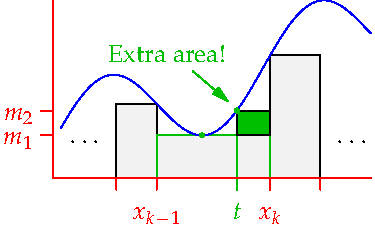
\includegraphics[scale=0.95]{riemann-sum3}
	\end{minipage}
	\par\vspace{-17pt}
	
	\begin{enumerate}\setcounter{enumi}{1}
	  \item[]\begin{align*}
	  	\textcolor{Green}{L(f,Q)-L(f,P)} 
	  	&=m_1(t-x_{k-1}) +m_2(x_{k}-t) -m(x_k-x_{k-1})\\
	  	&=(m_1-m)(t-x_{k-1}) +(m_2-m)(x_k-t)
	  	\mathrel{\textcolor{Green}{\ge 0}}
	  \end{align*}
	  More generally, since a refinement $Q$ is obtained by adding \emph{finitely many} new points, induction tells us that $P\subseteq Q\Longrightarrow L(f,P)\le L(f,Q)$.\smallbreak
	  The argument for $U(f,Q)\le U(f,P)$ is similar, and the middle inequality is trivial.
	  
	  \item If $P$ and $Q$ are partitions, then $P\cup Q$ is a refinement of both $P$ and $Q$. By part 1,
	  \[
	  	L(f,P)\le L(f,P\cup Q)\le U(f,P\cup Q)\le U(f,Q)\tag{$\ast$}
	  \]
	  
		\item This is an exercise.\qedhere
	\end{enumerate}
\end{proof}


\begin{thm}{}{partitionseq}
	Suppose $f:[a,b]\to\R$ is bounded.
	\begin{enumerate}
	  \item\label{thm:partitionseq1} (Cauchy criterion)\lstsp $f$ is integrable $\Longleftrightarrow\forall\epsilon>0$, $\exists P$ such that $U(f,P)-L(f,P)<\epsilon$.
	  \item $f$ is integrable $\Longleftrightarrow\exists (P_n)_{n\in\N}$ such that $U(f,P_n)-L(f,P_n)\to 0$. In such a situation, both sequences $U(f,P_n)$ and $L(f,P_n)$ converge to $\int_a^bf$.
	\end{enumerate} 
\end{thm}

Part 1 is termed a `Cauchy' criterion since it doesn't mention the integral (limit). 


\begin{proof}
	We prove the Cauchy criterion, leaving part 2 as an exercise. 
	\begin{description}
		\item[$(\Rightarrow)$] Suppose $f$ is integrable and that $\epsilon>0$ is given. Since $\inf U(f,Q)=\int f=\sup L(f,R)$, there exist partitions $Q,R$ such that
		\[
			U(f,Q)<\int f+\frac\epsilon 2
			\quad\text{and}\quad 
			L(f,R)>\int f-\frac \epsilon 2
		\]
		Let $P=Q\cup R$ and apply ($\ast$): \ $L(f,R)\le L(f,P)\le U(f,P)\le U(f,Q)$. But then
		\[
			U(f,P)-L(f,P)\le U(f,Q)-L(f,R) 
			=U(f,Q)-\int f+\int f-L(f,R)<\epsilon
		\]
		\item[$(\Leftarrow)$] Assume the right hand side. For every partition, $L(f,P)\le L(f)\le U(f)\le U(f,P)$. Thus
		\[
			0\le U(f)-L(f)\le U(f,P)-L(f,P)<\epsilon
		\]
		Since this holds for all $\epsilon>0$, we see that $U(f)=L(f)$: that is, $f$ is integrable.\qedhere
	\end{description}
\end{proof}

\goodbreak


\begin{examples}{}{riemannint2}
	\exstart Consider $f(x)=\sqrt x$ on the interval $[0,b]$. We choose a sequence of partitions $(P_n)$ that evaluate nicely when fed to this function:
	\begin{gather*}
	  P_n=\{x_0,\ldots,x_n\}\quad\text{where}\quad x_i=\left(\frac in\right)^2b\\
	  \implies \Delta x_i=x_i-x_{i-1}=\frac b{n^2}\bigl(i^2-(i-1)^2\bigr)=\frac{(2i-1)b}{n^2}
	\end{gather*}
	Since $f$ is increasing on $[0,b]$, we see that
	\begin{align*}
	  U(f,P_n)
	  &=\sum_{i=1}^nf(x_i)\Delta x_i 
	  	=\sum_{i=1}^n\frac{i\sqrt b}n\cdot\frac{(2i-1)b}{n^2} 
	  	=\frac{b^{3/2}}{n^3}\sum_{i=1}^n2i^2-i \\
	  &=\frac{b^{3/2}}{n^3}\left[\frac 13n(n+1)(2n+1)-\frac 12n(n+1)\right] 
	  	\xrightarrow[n\to\infty]{}\frac 23b^{3/2}
	\end{align*}
	Similarly
	\begin{align*}
	  L(f,P_n)
	  &=\sum_{i=1}^nf(x_{i-1})\Delta x_i 
	  	=\sum_{i=1}^n\frac{(i-1)\sqrt b}n\cdot\frac{(2i-1)b}{n^2} 
	  	=\frac{b^{3/2}}{n^3}\sum_{i=1}^n2i^2-3i+1 \\
	  &=\frac{b^{3/2}}{n^3}\left[\frac 13n(n+1)(2n+1)-\frac 32n(n+1) +n\right] 
	  	\xrightarrow[n\to\infty]{}\frac 23b^{3/2}
	\end{align*}
	Since the limits are equal, we conclude that $f$ is integrable and $\int_0^b\sqrt x\,\dx=\frac 23b^{3/2}$.
	
	\begin{enumerate}\setcounter{enumi}{1}
	  \item[]\begin{center}
		  \begin{tabular}{c@{\qquad}c}
		  	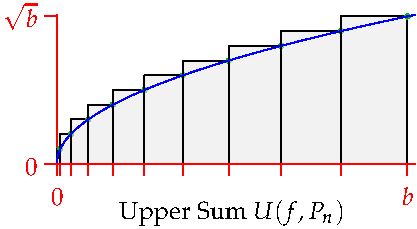
\includegraphics[scale=0.95]{darboux-ex1}
		  	&
		  	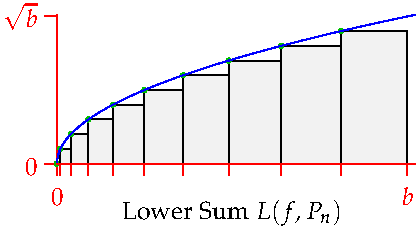
\includegraphics[scale=0.95]{darboux-ex2}
	  	\end{tabular}
	  \end{center}
	  
		\item\label{ex:riemannint2nonint} Here is the classic example of a \emph{non-integrable function}. Let $f:[a,b]\to\R$ to be the indicator function of the irrational numbers,
		\[
			f(x)=
			\begin{cases}
				1&\text{if }x\not\in\Q\\
				0&\text{if }x\in\Q
			\end{cases}
		\]
		Suppose $P=\{x_0,\ldots,x_n\}$ is \emph{any} partition of $[a,b]$. Since any interval of positive length contains both rational and irrational numbers, we see that
		\begin{gather*}
			\sup\bigl\{f(x):x\in[x_{i-1},x_i]\bigr\} =1 \implies U(f,P)=\sum_{i=1}^n(x_i-x_{i-1})=b-a\implies U(f)=b-a\\
			\inf\bigl\{f(x):x\in[x_{i-1},x_i]\bigr\}=0 \implies L(f,P)=0\implies L(f)=0
		\end{gather*}
		Since the upper and lower Darboux integrals differ, $f$ is not (Riemann) integrable.
	\end{enumerate}
\end{examples}


% \begin{asidep}
% The definition we have given is strictly that of the \emph{Darboux integral}. Riemann's definition is as follows:
% 
% \begin{defn}
% Let $f$ be bounded on $[a,b]$ and let $P$ be a partition. A \emph{Riemann sum} of $f$ associated to $P$ is a sum
% \[\sum_{k=1}^nf(x_k)(t_k-t_{k-1}),\text{ where }x_k\in[t_{k-1},t_k].\]
% $f$ is \emph{Riemann integrable} on $[a,b]$ with integral $r$ if for all $\epsilon>0$ there exists $\delta>0$ such that for all Riemann sums $S$ with partitions finer than $\delta$ (i.e. $t_k-t_{k-1}<\delta$ for all $k$) we have
% \[\nm{S-r}<\epsilon.\]
% \end{defn}
% 
% It is common to use the term Riemann integral for either Riemann's or Darboux's definition since they coincide (by contrast, alternative definitions of the integral allow more functions to be considered integrable). Indeed we have the following theorem:
% 
% \begin{thm}
% $f$ is Riemann integrable on $[a,b]$ iff it is Darboux integrable on $[a,b]$, in which case the values of the integrals coincide.
% \end{thm}
% 
% In order to prove the theorem, and several others in the next section, it is convenient to have the following definition and $\epsilon$--$\delta$ criterion for integrability, which we state without its uninstructive proof.
% 
% \begin{defn}
% Given a partition $P=\{t_0<\cdots<t_n\}$ of $[a,b]$, the \emph{mesh} of $P$ is the maximum of the distances between successive $t_k$. I.e. $\mesh(P)=\max(t_k-t_{k-1})$.
% \end{defn}
% 
% \begin{prop}\label{prop:intepsilon}
% A bounded function $f$ on $[a,b]$ is integrable iff either of the following conditions hold:
% \begin{enumerate}
%   \item For each $\epsilon>0$ there exists a partition $P$ of $[a,b]$ such that
% \[U(f,P)-L(f,P)<\epsilon.\]
% \item For all $\epsilon>0$ there exists $\delta>0$ such that
% \[\mesh(P)<\delta\Longrightarrow U(f,P)-L(f,P)<\epsilon.\]
% \end{enumerate}
% \end{prop}
% 
% The proposition is intuitive in the sense that we visualize the upper and lower Darboux sums as converging to the integral. This is, of course, not technically correct, since there is no sequence of Darboux sums.
% 
% \begin{proof}[Proof of Theorem]
% Suppose $f$ is Darboux integrable and let $\epsilon>0$ be chosen. Let $\delta>0$ be chosen satisfying Proposition \ref{prop:intepsilon}. Let $P$ be any partition of $[a,b]$ with $\mesh(P)<\delta$ and let $S$ be a Riemann sum associated to $P$. Clearly we have
% \[L(f,P)\le S\le U(f,P).\]
% By Proposition \ref{prop:intepsilon} we have
% \[U(f,P)<L(f,P)+\epsilon\le L(f)+\epsilon.\]
% Similarly
% \[L(f,P)>U(f,P)-\epsilon\ge U(f)-\epsilon.\]
% Since $U(f)=L(f)=\int_a^bf$ we see that
% \[\int_a^bf-\epsilon<S<\int_a^b+\epsilon.\]
% Hence $f$ is Riemann integrable, with integral $r=\int_a^bf$.\\
% Now suppose $f$ is Riemann integrable with integral $r$. Let $\epsilon>0$ be given, $\delta>0$ satisfying the definition and $P$ a partition finer than $\delta$. Then any Riemann sum associated to $P$ satisfies
% \[\nm{S-r}<\epsilon.\]
% Since $\epsilon>0$ we may select $x_k\in[t_{k-1},t_k]$ such that
% \[f(x_k)>\sup\{f(x):x\in[t_{k-1},t_k]\}-\epsilon.\]
% The Riemann sum $S$ for these $x_i$ clearly satisfies
% \[S\ge U(f,P)-\epsilon(b-a).\]
% But then, for all $\epsilon>0$ we have
% \[U(f)\le U(f,P)\le S+\epsilon(b-a)\le r+\epsilon+\epsilon(b-a)=r+\epsilon(1+b-a),\]
% so that $U(f)\le r$. Similarly we see that $L(f)\ge r$. Then $U(f)\ge L(f)$ implies equality and so $f$ is Darboux integrable with integral $\int_a^bf=r$.
% \end{proof}
% \end{asidep}\newpage

As any freshman calculus student can attest, if you can find an anti-derivative, then the fundamental theorem of calculus (Section \ref{sec:ftc}) makes evaluating integrals far easier. For instance, you are probably desperate to write
\[
	\diff x\frac 23x^{3/2}=x^{1/2}
	\implies \int_0^b\sqrt x\,\dx
	=\frac 23x^{3/2}\Big|_0^b
	=\frac 23b^{3/2}
\]
rather than computing Riemann/Darboux sums as in the previous example! However, in most practical situations, no easy-to-compute anti-derivative exists; the best we can do is to approximate using Riemann sums for progressively finer partitions. Thankfully computers excel at such tedious work!


\begin{exercises}
	\emph{Key concepts:\quad Darboux sums/integrals,\qquad Partitions, sample points \& refinements,}
	\begin{quote}
		\emph{Cauchy \& sequential criteria for integrability}
	\end{quote}
	
	\begin{enumerate}
		\item\label{exs:easydarbint} Use partitions to find the upper and lower Darboux integrals on the interval $[0,b]$. Hence prove that the function is integrable and compute its integral.
		\begin{enumerate}
		  \item $f(x)=x^3$\qquad\qquad\qquad (b) \ $g(x)=\sqrt[3]{x}$%\par
		  %(\emph{Hint: mimic Example \hyperref[ex:riemannint2]{\ref*{ex:riemannint2}.1})}
		\end{enumerate}
		
		
		\item Repeat question \ref*{exs:easydarbint} for the following two functions. You cannot simply compute Riemann sums for left and right endpoints and take limits: why not?
		\begin{enumerate}  
		  \item $h(x)=x(2-x)$ on $[0,2]$\smallbreak
		  (\emph{Hint: choose a partition with $2n$ subintervals such that $x_n=1$ and observe that $h(2-x)=h(x)$})
		  
		  \item On the interval $[0,3]$, let $k(x)=\begin{cases}
		  2x&\text{if }x\le 1\\
		 	5-x&\text{if }x>1
		  \end{cases}$\smallbreak
		  (\emph{Hint: this time try a partition with $3n$ subintervals})
		\end{enumerate}
	
	
	  \item Let $f(x)=x$ for rational $x$ and $f(x)=0$ for irrational $x$. Calculate the upper and lower Darboux integrals for $f$ on the interval $[0,b]$. Is $f$ integrable on $[0,b]$?
	
	    
		\item Prove part 3 of Lemma \ref{lemm:partitionseqlemm}: $L(f)\le U(f)$.
	
	
		\item Prove part 2 of Theorem \ref{thm:partitionseq}.
	 	\begin{quote}
	 		$f$ is integrable $\iff\exists (P_n)_{n\in\N}$ such that $\lim\limits_{n\to\infty}\bigl(U(f,P_n)-L(f,P_n)\bigr) =0$
	 	\end{quote}
	 	Moreover, prove that both $U(f,P_n)$ and $L(f,P_n)$ converge to $\int f$.
		
		\item\begin{enumerate}
		  \item Reread Definition \ref{defn:darbouxint}. What happens if we allow $f:[a,b]\to\R$ to be \emph{unbounded}?
		  \item (Hard)\lstsp Read ``\emph{Riemann versus Darboux}'' on page \pageref{pg:riemanndefthm}. Explain why being \emph{Riemann} integrable also forces $f$ to be bounded.
		  \item (Hard)\lstsp Explain the observation that $L(f,P)$ is the infimum of the set of all Riemann sums on $P$.
		\end{enumerate}
	
		\item (If you like coding)\quad Write a short program to estimate $\int_a^bf(x)\,\dx$ using Riemann sums. This can be very simple (equal partitions with right endpoints), or more complex (random partition and sample points given a mesh). Apply your program to estimate $\int_0^{5}\sin(x^2e^{-\sqrt x})\,\dx$.
	\end{enumerate}
\end{exercises}



\clearpage



\subsection{Properties of the Riemann Integral}\label{sec:riemannproperties}

The rough take-away of this long section is that everything you think is integrable probably is! Examples will be few, since we have not established many explicit values for integrals.


\begin{thm}{Linearity}{intlinear}
	If $f,g$ are integrable and $k,l$ are constant, then $kf+lg$ is integrable and
	\[
		\int  kf+lg=k\int f+l\int g
	\]
\end{thm}

\begin{example}{}{}
Thanks to examples in the previous section, we can now calculate, e.g.,
\[
	\int_0^25x^3-3\sqrt x\,\dx
	=5\cdot\frac 14\cdot 2^4 -3\cdot \frac 23\cdot 2^{3/2} 
	=20-4\sqrt 2
\]
\end{example}

\begin{proof}
	Suppose $\epsilon>0$ is given. By the Cauchy criterion (Theorem \ref{thm:partitionseq}, part \ref*{thm:partitionseq1}), there exist partitions $R,S$ such that
	\[
		U(f,R)-L(f,R)<\smash{\frac\epsilon 2}
		\quad\text{and}\quad 
		U(g,S)-L(g,S)<\smash{\frac\epsilon 2}
	\]
	If $P=R\cup S$, then both inequalities are satisfied by $P$ (Lemma \ref{lemm:partitionseqlemm}). On each subinterval,
	\[
		\inf f(x)+\inf g(x)\le \inf\bigl(f(x)+g(x)\bigr)
		\quad\text{and}\quad 
		\sup\bigl(f(x)+g(x)\bigr)\le\sup f(x)+\sup g(x)
	\]
	since the individual suprema/infima could be `evaluated' at different places. Thus
	\[
		L(f,P)+L(g,P)\le L(f+g,P)\le U(f+g,P)\le U(f,P)+U(g,P)
	\]
	whence $U(f+g,P)-L(f+g,P)<\epsilon$ and $f+g$ is integrable. Moreover,
	\[
		\int(f+g)-\int f-\int g \le \Bigl(U(f,P)-\int f\Bigr)+\Bigl(U(g,P)-\int g\Bigr)<\epsilon
	\]
	Using lower Darboux integrals similarly obtains the other half of the inequality
	\[
		-\epsilon<\int(f+g)-\int f-\int g<\epsilon
	\]
	Since this holds for all $\epsilon>0$, we conclude that $\int(f+g)=\int f+\int g$.\smallbreak
	That $kf$ is integrable with $\int kf=k\int f$ is an exercise. Put these together for the result.
\end{proof}


\begin{cor}{Changing endvalues}{intopen}
	Suppose $f$ is integrable on $[a,b]$ and $g:[a,b]\to\R$ satisfies $f(x)=g(x)$ on $(a,b)$. Then $g$ is also integrable on $[a,b]$ and $\int_a^b g=\int_a^b f$.
\end{cor}


\begin{defn}{Integration on an open interval}{intopen}
	A \emph{bounded} function $g:(a,b)\to\R$ is \emph{integrable} if it has an integrable extension $f:[a,b]\to\R$ where $f(x)=g(x)$ on $(a,b)$.
	In such a case, we define $\int_a^bg:=\int_a^bf$.
\end{defn}

The Corollary (its proof is an exercise) shows that the choice of extension is irrelevant.


\goodbreak


\begin{thm}{Basic integral comparisons}{intineq}
	Suppose $f$ and $g$ are integrable on $[a,b]$. Then:
	\begin{enumerate}\itemsep1pt\parsep=1pt
	  \item $f(x)\le g(x) \Longrightarrow\int f\le\int g$
	  \item $m\le f(x)\le M\Longrightarrow m(b-a)\le\int_a^bf\le M(b-a)$
	  \item $fg$ is integrable.
	  \item $\nm f$ is integrable and $\nm{\int f}\le\int \nm f$
	  \item $\max(f,g)$ and $\min(f,g)$ are both integrable.
	\end{enumerate}
\end{thm}

Part 3 is \emph{not} integration by parts since it doesn't tell us how $\int fg$ relates to $\int f$ and $\int g$!

\begin{proof}
	\begin{enumerate}\itemsep=1pt\parsep=1pt
	  \item Since $g-f$ is positive and integrable, $L(g-f,P)\ge 0$ for all partitions $P$. But then
	  \[
	  	\smash{0\le \inf L(g-f,P)=L(g-f)=\int g-f=\int g-\int f}
	  \]
	  \item Apply part 1 twice.
	  \item This is an exercise.
	  \item The integrability is an exercise. For the comparison, apply part 1 to $-\nm f\le f\le\nm f$.
	  \item Use $\max(f,g)=\frac 12(f+g)+\frac 12\nm{f-g}$, etc., together with the previous parts.\qedhere
	\end{enumerate}
\end{proof}


\begin{thm}[lower separated=false, sidebyside, sidebyside align=top seam, sidebyside gap=0pt, righthand width=0.35\linewidth]{Domain splitting}{domainsplit}
	Suppose $f:[a,b]\to\R$ and let $c\in(a,b)$. If $f$ is integrable on both $[a,c]$ and $[c,b]$, then it is integrable on $[a,b]$ and
	\[
		\int_a^bf=\int_a^cf+\int_c^bf
	\]
	\tcblower
	\flushright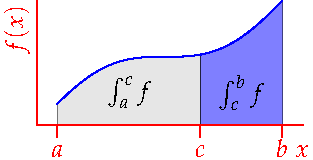
\includegraphics[scale=0.95]{domain-split}
\end{thm}

In light of this result, it is conventional to allow integral limits to be reversed: if $a<b$, then
\[
	\int_b^af:=-\int_a^bf
	\quad\text{ is consistent with }\quad 
	\int_a^af=0
\]


\begin{proof}
	Let $\epsilon>0$ be given, then $\exists R,S$ partitions of $[a,c],[c,b]$ such that\par
	\begin{minipage}[t]{0.65\linewidth}\vspace{-10pt}
		\[
			U(f,R)-L(f,R)<\frac\epsilon 2,\qquad U(f,S)-L(f,S)<\frac\epsilon 2
		\]
		Choose $P=R\cup S$ to partition $[a,b]$, then
		\[
			U(f,P)-L(f,P)=U(f,R)+U(f,S)-L(f,R)-L(f,S)<\epsilon
		\]
		Moreover
	\end{minipage}
	\hfill
	\begin{minipage}[t]{0.34\linewidth}\vspace{0pt}
		\flushright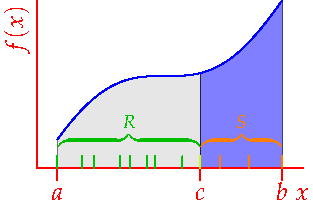
\includegraphics[scale=0.95]{domain-split2}
	\end{minipage}\par
	\[
		\int_a^bf-\int_a^cf-\int_c^bf
		\le U(f,P)-L(f,R)-L(f,S)
		=U(f,P)-L(f,P)<\epsilon
	\]
	Showing that this expression is greater than $-\epsilon$ is similar.
\end{proof}


\goodbreak


\begin{example}{}{}
	If $f(x)=\sqrt x$ on $[0,1]$ and $f(x)=1$ on $[1,2]$, then
	\[
		\int_0^2f =\int_0^1\sqrt x\,\dx+\int_1^2 1\,\dx
		=\frac 23+1 =\frac 53
	\]
\end{example}


\boldinline{Monotonic \& Continuous Functions}

We establish the integrability of two large classes of functions.

\begin{defn}{}{}
	A function $f:[a,b]\to\R$ is:
	\begin{description}\itemsep1pt
		\item[\normalfont\emph{Monotonic}] if it is either \emph{increasing} ($x<y\Longrightarrow f(x)\le f(y)$) or \emph{decreasing}.
		\item[\normalfont\emph{Piecewise monotonic}] if there is a partition $P=\{x_0,\ldots,x_n\}$ (finite!) of $[a,b]$ such that $f$ is monotonic on each open subinterval $(x_{k-1},x_k)$.
		\item[\normalfont\emph{Piecewise continuous}] if there is a partition such that $f$ is \emph{uniformly continuous} on each $(x_{k-1},x_k)$.
	\end{description}
\end{defn}


\begin{thm}{}{monotoneint}
	If $f$ is \emph{monotonic} or \emph{continuous} on $[a,b]$, then it is integrable.
\end{thm}


\begin{examples}{}{}
	\exstart Since sine is continuous, we can approximate via a sequence of Riemann sums
	\[
		\int_0^\pi\sin x\,\dx 
		=\frac\pi{n}\lim_{n\to\infty}\sum_{i=1}^n\sin\frac{\pi i}n
	\]
	\emph{Evaluating} this limit is another matter entirely, one best handled in the next section...\vspace{-3pt}
	\begin{enumerate}\setcounter{enumi}{1}
	  \item Similarly, $e^{\sqrt x}$ is integrable and therefore may be approximated via Riemann sums:
	  \[
	  	\int_0^1 e^{\sqrt x}\,\dx 
	  	=\frac 1{n}\lim\limits_{n\to\infty}\sum_{i=1}^n \exp\sqrt{\frac in} 
	  	=\lim\limits_{n\to\infty}\sum_{j=1}^n \frac{2j-1}n\exp\frac jn
	  \]
	  Both sums use right endpoints: the first has equal subintervals, while the second is analogous to Example \ref{ex:riemannint2}.1. These limits would typically be estimated using a computer.
	\end{enumerate}
\end{examples}

\begin{proof}
	Since $[a,b]$ is closed and bounded, a continuous function $f$ is \emph{uniformly} so. Let $\epsilon>0$ be given:
	\[
		\exists\delta>0\text{ such that }
		\forall x,y\in[a,b],\ 
		\nm{x-y}<\delta \implies \nm{f(x)-f(y)}<\frac\epsilon{b-a}
	\]
	Let $P$ be a partition with $\mesh P<\delta$. Since $f$ attains its bounds on each $[x_{i-1},x_i]$,
	\[
		\exists x_i^*,y_i^*\in [x_{i-1},x_i]
		\quad\text{such that}\quad 
		M_i-m_i=f(x_i^*)-f(y_i^*)<\frac\epsilon{b-a}
	\]
	from which
	\[
		U(f,P)-L(f,P)
		<\smash[t]{\sum_{i=1}^n}\frac\epsilon{b-a}(x_i-x_{i-1})
		=\epsilon
	\]
	The monotonicity argument is an exercise.
\end{proof}

Combining the proof with Definition \ref{defn:intopen}: every \emph{uniformly continuous} $f:(a,b)\to\R$ is integrable.

\goodbreak


\begin{cor}{}{piecewiseint}
	Piecewise continuous and \textbf{bounded} piecewise monotonic functions are integrable.
\end{cor}


\begin{proof}
	If $f$ is piecewise continuous, then the restriction of $f$ to $(x_{k-1},x_k)$ has a continuous extension $g_k:[x_{k-1},x_k]\to\R$; this is integrable by Theorem \ref{thm:monotoneint}. By Corollary \ref{cor:intopen}, $f$ is integrable on $[x_{k-1},x_k]$ with $\int_{x_{k-1}}^{x_k}f=\int_{x_{k-1}}^{x_k}g_k$. Theorem \ref{thm:domainsplit} ($n-1$ times!) finishes things off:
	\[
		\int_a^bf=\sum_{k=1}^n\int_{x_{k-1}}^{x_k}f
	\]
	The argument for piecewise monotonicity is similar.
\end{proof}


\begin{example}[lower separated=false, sidebyside, sidebyside align=top seam, sidebyside gap=0pt, righthand width=0.35\linewidth]{}{fracpart}
	The `fractional part' function $f(x)=x-\lfloor x\rfloor$ is both piecewise continuous and piecewise monotone on any bounded interval. It is therefore integrable on any such interval.
	\tcblower
	\flushright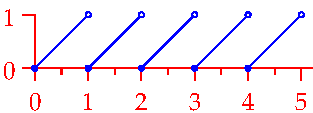
\includegraphics{fracpart}
\end{example}


For a final corollary, here is one more incarnation of the intermediate value theorem.

\begin{cor}{IVT for integrals}{}
	If $f$ is continuous on $[a,b]$, then $\exists \xi\in (a,b)$ for which
	\[
		f(\xi)=\frac 1{b-a}\int_a^bf
	\]
\end{cor}

\begin{proof}
	Since $f$ is continuous, it is integrable on $[a,b]$. By the extreme value theorem it is also bounded and attains its bounds: $\exists p,q\in[a,b]$ such that\par
	\begin{minipage}[t]{0.55\linewidth}\vspace{-5pt}
		\[
			f(p):=\inf\limits_{x\in[a,b]}f(x),\qquad f(q)=\sup\limits_{x\in[a,b]}f(x)
		\]
		Applying Theorem \ref{thm:intineq}, part 2, with $m=f(p)$ and $M=f(q)$, we see that
		\[
			(b-a)f(p)\le\int_a^bf\le (b-a)f(q)
		\]
	\end{minipage}
	\hfill
	\begin{minipage}[t]{0.44\linewidth}\vspace{-5pt}
		\flushright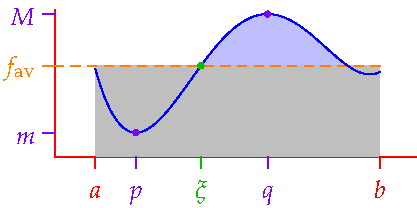
\includegraphics[scale=0.95]{average}
	\end{minipage}\bigbreak

	Divide by $b-a$ and apply the usual intermediate value theorem for $f$ to see that the required $\xi$ exists between $p$ and $q$.
\end{proof}

In the picture, when $f$ is positive and continuous, the grey area equals that under the curve; imagine levelling off the blue hill with a bulldozer\ldots{} The notation $\textcolor{orange}{f_{\text{av}}}=\frac 1{b-a}\int_a^bf$ indicates the \textcolor{orange}{average value} of $f$ on $[a,b]$: to see why this interpretation is sensible, take a sequence of Riemann sums on equally-spaced partitions $P_n$ to see that
\[
	\frac 1{b-a}\int_a^b f 
	=\lim_{n\to\infty}\sum_{i=1}^nf(x_i^*)\Delta x
	=\lim_{n\to\infty}\frac{f(x_1^*)+\cdots+f(x_n^*)}n
\]
is the limit of a sequence of \emph{averages} of equally-spaced samples $f(x_i^*)$.


\goodbreak


\boldsubsubsection{What can/cannot be integrated?}

We now know a great many examples of integrable functions:
\begin{itemize}\itemsep0pt
  \item Piecewise continuous \& monotonic functions are integrable.
  \item Linear combinations, products, absolute values, maximums and minimums of (already) integrable functions.
\end{itemize}

By contrast, we've only seen one non-integrable function (Example \ref*{ex:riemannint2}.\ref{ex:riemannint2nonint}). After so many positive integrability conditions, it is reasonable to ask precisely which functions are Riemann integrable. Here is the answer, though it is quite tricky to understand.

\begin{thm}{Lebesgue}{lebesgue}
	Suppose $f:[a,b]\to\R$ is bounded. Then
	\begin{quote}
		$f$ is Riemann integrable $\iff$ it is continuous except on a set of \emph{measure zero}
	\end{quote}
\end{thm}

Naïvely, the \emph{measure} of a set is the sum of the lengths of its maximal subintervals, though unfortunately this doesn't make for a very useful definition.\footnote{%
	Formally, the \emph{length} of an open interval $(a,b)$ is $b-a$ and a set $A\subseteq \R$ has \emph{measure zero} if
	\[
		\forall\epsilon>0,\ \exists \text{ open intervals $I_n$ such that }
		A\subseteq\bigcup_{n=1}^\infty I_n
		\text{ and }
		\sum_{i=1}^\infty\operatorname{length}(I_n)<\epsilon
	\]
	More generally, the \emph{Lebesgue measure} of a set (subject to a technical condition) is the infimum of the sum of the lengths of any countable collection of open covering intervals. \emph{Measure theory} is properly a matter for graduate study.	Surprisingly, there exist \href{https://en.wikipedia.org/wiki/Smith-Volterra-Cantor_set}{sets} with positive measure that contain no subintervals, and even sets which are non-measurable!%
}
Any countable subset has measure zero, so Lebesgue's result is almost as if we can extend Corollary \ref{cor:piecewiseint} to allow for infinite sums. For instance, Exercise \ref*{sec:cont}.\ref{exs:discontq} describes a function which is continuous only on the irrationals: it is thus Riemann integrable (indeed $\int_a^bf=0$ for any $a<b$). There are also uncountable sets with measure zero such as Cantor's middle-third set $\mathcal C$: the function
\[
	f(x)=
	\begin{cases}
		1&\text{if }x\in\mathcal C\\
		0&\text{otherwise}
	\end{cases}
\]
is continuous except on $\mathcal C$ and therefore Riemann integrable; again $\int_0^1 f(x)\,\dx=0$.


\vfil

\begin{exercises}
	\emph{Key concepts:\quad Linear combinations, products, etc., of integrable functions are integrable,}\vspace{-5pt}
 	\begin{quote}
 		\emph{Continuous and monotone functions are integrable,\qquad Integrability on open intervals}
 	\end{quote}


	\begin{enumerate}
	  \item Explain why $\int_{0}^{2\pi}x^2\sin^8(e^x)\,\dx \le\frac 83\pi^3$
	  
	  
		\item If $f$ is integrable on $[a,b]$ prove that it is integrable on any interval $[c,d]\subseteq[a,b]$.
		
		
		\item We complete the proof of Theorem \ref{thm:intlinear} (linearity of integration).
		\begin{enumerate}
	  	\item Suppose $k>0$, let $A\subseteq\R$ and define $kA:=\{kx:x\in A\}$. Prove that $\sup kA=k\sup A$ and $\inf kA=k\inf A$.
	  	\item If $k>0$ prove that $kf$ is integrable on any interval and that $\int kf=k\int f$.
	  	\item How should you modify your argument if $k<0$?
		\end{enumerate}
		
	  
	  \item Give an example of an integrable but \emph{discontinuous} function on a closed bounded interval $[a,b]$ for which the conclusion of the Intermediate Value Theorem for Integrals is \emph{false.}
	  
	  
		\item Use Darboux sums to compute the value of the integral $\int_{1/2}^{{15/2}} x-\lfloor x\rfloor \,\dx$ (Example \ref{ex:fracpart}).
		
		
		\item\label{exs:extensionlemma} We prove and extend Corollary \ref{cor:intopen}. Suppose $f$ is integrable on $[a,b]$. 
		\begin{enumerate}
		  \item If $g:[a,b]\to\R$ satisfies $f(x)=g(x)$ for all $x\in (a,b)$, prove that $g$ is integrable and $\int_a^bg=\int_a^bf$.\smallbreak
			(\emph{Hint: consider $h=f-g$ and show that $\int h=0$})
			\item Now suppose $g:[a,b]\to\R$ satisfies $f(x)=g(x)$ for all $x\in [a,b]$ except at finitely many points. Prove that $g$ is integrable and $\int_a^bg=\int_a^bf$.
		\end{enumerate}
	  
	  
	  \item Show that an increasing function on $[a,b]$ is integrable and thus complete Theorem \ref{thm:monotoneint}.\par
	  (\emph{Hint: Choose a partition with $\mesh P<\frac\epsilon{f(b)-f(a)}$})
	 
	  
	  \item Suppose $f$ and $g$ are integrable on $[a,b]$.
		\begin{enumerate}
	    \item Define $h(x)=\bigl(f(x)\bigr)^2$. We know:
	  	\begin{itemize}
	    	\item $f$ is bounded: $\exists K$ such that $\nm{f(x)}\le K$ on $[a,b]$.
	    	\item Given $\epsilon>0$, $\exists P$ such that $U(f,P)-L(f,P)<\frac\epsilon{2K}$.
	  		For each subinterval $[x_{i-1},x_i]$, let
	  		\[
	  			M_i=\sup f(x),\qquad m_i=\inf f(x),\qquad 
	  			\cl M_i=\sup h(x),\qquad \cl m_i=\inf h(x)
	  		\]
	  	\end{itemize}
	  	Prove that $\cl M_i-\cl m_i\le 2(M_i-m_i)K$. Hence conclude that $h$ is integrable.
	  	
	  	\item Prove that $fg$ is integrable.\par
	  	(\emph{Hint: $fg=\frac 14(f+g)^2-\frac 14(f-g)^2$})
	  	
	  	\item Prove that $U(\nm f,P)-L(\nm f,P)\le U(f,P)-L(f,P)$ for any partition $P$. Hence conclude that $\nm f$ is integrable.
	  \end{enumerate}

	  (\emph{One can extend these arguments to show that if $j$ is continuous, then $j\circ f$ is integrable. Parts (a) and (c) correspond, respectively, to $j(x)=x^2$ and $j(x)=\nm x$.})
	  
	  
	  \item (Hard)\quad Let $f(x)=
	  \begin{cases}
	  	x&\text{if }x\neq 0\text{ and }\sin\frac 1x>0\\
	  	-x&\text{if }x\neq 0\text{ and }\sin\frac 1x<0\\
	  	0&\text{if }x=0 
	  \end{cases}$
	  \begin{enumerate}
	  	\item Show that $f$ is not piecewise continuous on $[0,1]$.
	  	
	    \item Show that $f$ is not piecewise monotonic on $[0,1]$.
	    
	    \item Show that $f$ is integrable on $[0,1]$.\par
	    (\emph{Hint: given $\epsilon$, hunt for a suitable partition to make $U(f,P)-L(f,P)<\epsilon$ by considering $[0,x_1]$ differently to the other subintervals})
	    
	    \item Make a similar argument which proves that $g=\sin\frac 1x$ is integrable on $(0,1]$.\par
	    (\emph{Hint: Show that $g$ has an integrable extension on $[0,1]$})
	  \end{enumerate}
	
	\end{enumerate}
\end{exercises}


\clearpage


\subsection{The Fundamental Theorem of Calculus}\label{sec:ftc}

The key result linking integration and differentiation is usually presented in two parts. While there are significant subtleties, the rough statements are as follows (we follow the traditional numbering):

\begin{description}
	\item[\normalfont\emph{Part I} ] Differentiation reverses integration: $\diff x\int_a^xf(t)\,\dt=f(x)$
	\item[\normalfont\emph{Part II} ] Integration reverses differentiation: $\int_a^bF'(x)\,\dx =F(b)-F(a)$
\end{description}

\begin{minipage}[t]{0.7\linewidth}\vspace{-10pt}
	These facts seemed intuitively obvious to early practitioners of calculus. Given a continuous positive function $f$:
	\begin{itemize}
	  \item Let $F(x)$ denote the area under $y=f(x)$ between $0$ and $x$. 
	  \item A small increase $\Delta x$ results in the area increasing by $\Delta F$.
	  \item $\Delta F\approx f(x)\Delta x$ is approximately the area of a rectangle, whence $\frac{\Delta F}{\Delta x}\approx f(x)$. This is part I.
	  \item $F(b)-F(a)\approx\sum \Delta F_i\approx \sum f(x_i)\Delta x_i$. Since $F'=f$, this is part II.
	\end{itemize}
\end{minipage}
\hfill
\begin{minipage}[t]{0.29\linewidth}\vspace{-10pt}
	\flushright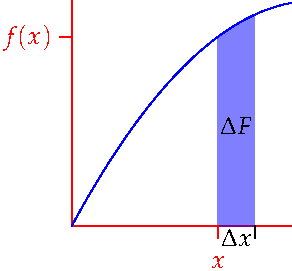
\includegraphics[scale=0.95]{ftcold}
\end{minipage}\medbreak

When Leibniz introduced the symbols $\int$ and $\D$ in the late 1600s, it was partly to reflect the fundamental theorem.\footnote{%
	\def\dF{\D F}$\int$ is a stylized S for \emph{sum,} while $\D$ stands for \emph{difference.} Given a sequence $F=(F_0,F_1,F_2,\ldots,F_n)$, construct a new sequence of \emph{differences}
	\[
		\dF=(F_1-F_0,F_2-F_1,\ldots,F_n-F_{n-1})
	\]
	which can then be summed:
	\[
		\int\dF=(F_1-F_0)+(F_2-F_1)+\cdots (F_n-F_{n-1})=F_n-F_0 \tag{$\ast$}
	\]
	Viewing a function as an `infinite sequence' of values spaced along an interval, $\dF$ becomes a sequence of \emph{infinitesimals} and $(\ast)$ is essentially the fundamental theorem: $\int\dF =F(b)-F(a)$. It is the concept of \textbf{function} that is suspect here, not the essential relationship between sums and differences.%
}
If you're happy with non-rigorous notions of limit, rate of change, area, and (infinite) sums, the above is all you need!\smallbreak
Of course we are very much concerned with the details: What must we assume about $f$ and $F$, and how are these properties used in the proof?

\begin{thm}{FTC, part I}{ftc1}
	Suppose $f$ is integrable on $[a,b]$. For any $x\in[a,b]$, define
	\[
		F(x):=\int_a^xf(t)\,\dt
	\]
	Then:
	\begin{enumerate}
	  \item $F$ is uniformly continuous on $[a,b]$;
	  \item If $f$ is continuous at $c\in[a,b]$, then $F$ is differentiable\footnotemark{} at $c$ with $F'(c)=f(c)$.
	\end{enumerate}
\end{thm}

\footnotetext{%
	Strictly: if $c=a$, then $F$ is \emph{right}-differentiable, etc.%
}

Compare this with the naïve version above where we assumed $f$ was continuous. We now require only the \emph{integrability} of $f$, and its continuity at \emph{one point} for the full result.


\goodbreak


\begin{examples}{}{ftc1}
	Examples in every elementary calculus course.
	\begin{enumerate}
	  \item Since $f(x)=\sin^2(x^3-7)$ is continuous on any bounded interval, we conclude that
	  \[
	  	\diff x\int_4^x\sin^2(t^3-7)\,\dt=\sin^2(x^3-7)
	  \]
	  If one follows Theorem \ref{thm:domainsplit} and its conventions, then this is valid for all $x\in\R$.
	  
	  
	  \item The chain rule permits more complicated examples. For instance: $f(t)=\sin\sqrt t$ is continuous on its domain $[0,\infty)$ and $y(x)=x^2+3$ has range $[3,\infty)\subseteq\dom(f)$, whence
	  \[
	  	\diff x\int_0^{x^2+3}\sin\sqrt t\,\dt 
	  	=\diff[y]{x}\diff y\int_0^{y}\sin\sqrt t\,\dt
	  	=2x\sin\sqrt{x^2+3}
	  \]
	  
	  
	  \item For a final positive example, we consider when
	  \[
			\diff x\int_{\sin x}^{e^x} \tan(t^2)\,\dt 
			=e^x\tan(e^{2x}) -\cos x\tan(\sin^2\!x)
		\]
	  Makes sense. To evaluate this, first choose any constant $a$ and write
	  \[
	  	\int_{\sin x}^{e^x} 
	  	=\int_a^{e^x}+\int_{\sin x}^a 
	  	=\int_a^{e^x}-\int_a^{\sin x}
	  \]
	  before differentiating. This is valid provided $\sin x$, $e^x$ and $a$ all lie in the same subinterval of
	  \[
	  	\dom\tan(t^2) =\R\setminus\{\pm\sqrt{\tfrac\pi 2},
	  	\pm\sqrt{\tfrac{3\pi}2},
	  	\pm\sqrt{\tfrac{5\pi}2},
	  	\ldots\}
	  \]
	  Since $\nm{\sin x}\le 1<\sqrt{\frac\pi 2}$, this requires
	  \[
	  	\nm{e^{2x}}<\frac\pi 2 \iff x<\frac 12\ln\frac\pi 2
	  \]
	  Choosing $a=1$ would certainly suffice.
	  
	  
	  \begin{minipage}[t]{0.7\linewidth}\vspace{0pt}
		  \item\label{ex:ftcdiscont} Now consider why the theorem requires continuity. The piecewise continuous function
		  \[
		  	f:[0,2]\to\R:x\mapsto
		  	\begin{cases}
		  		2x&\text{if }x\le 1\\
		  		\frac 12&\text{if }x>1
		  	\end{cases}
		 	\]
		  has a jump discontinuity at $x=1$. We can still compute
		  \[
		  	F(x)=
		  	\begin{cases}
		  		\int_0^x 2t\,\dt=x^2&\text{if }x\le 1\\
		  		\int_0^12t\,\dt+\int_1^x\frac 12\dt=\frac 12(x+1)&\text{if }x>1
		  	\end{cases}
		  \]
		  This is continuous, indeed uniformly so! However the discontinuity of $f$ results in $F$ having a \emph{corner} and thus being \emph{non-differentiable} at $x=1$. Indeed $F'(x)=f(x)$ whenever $x\neq 1$: that is, at all values of $x$ where $f$ is continuous.
	  \end{minipage}
	  \hfill
	  \begin{minipage}[t]{0.29\linewidth}\vspace{0pt}
	  	\flushright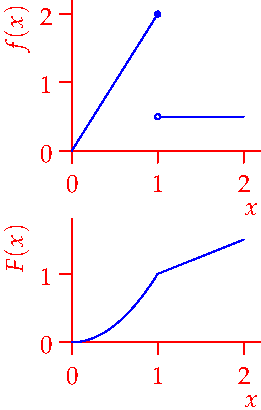
\includegraphics[scale=0.95]{ftc1}
	  \end{minipage}
	\end{enumerate}
\end{examples}


\goodbreak


\boldinline{Proving FTC\,I} Neither half of the theorem is particularly difficult once you write down what you know and what you need to prove. Here are the key ingredients:

\begin{enumerate}
  \item Uniform continuity for $F$ means we must control the size of
  \[
  	\nm{F(y)-F(x)}
  	=\nm{\int_a^yf(t)\,\dt-\int_a^xf(t)\,\dt}
  	=\nm{\int_x^yf(t)\,\dt}\le \int_x^y\nm{f(t)}\,\dt
  \]
  But the boundedness of $f$ allows us to control this last integral\ldots
  
  \item $F'(c)=f(c)$ means showing that $\lim\limits_{x\to c}\frac{F(x)-F(c)}{x-c}=f(c)$, which means controlling the size of
  \[
  	\nm{\frac{F(x)-F(c)}{x-c}-f(c)} =\nm{\frac 1{x-c}\int_{c}^xf(t)\,\dt-f(c)}
  \]
  The trick here will is to bring the \emph{constant} $f(c)$ inside the integral as $\frac 1{x-c}\int_c^xf(c)\,\dt$ so that the above becomes $\frac 1{\nm{x-c}}\int_c^x\nm{f(t)-f(c)}\,\dt$. This may now be controlled via the continuity of $f$\ldots
\end{enumerate}

\begin{proof}
	\begin{enumerate}
	  \item Since $f$ is integrable, it is bounded: $\exists M>0$ such that $\nm{f(x)}\le M$ for all $x$.\smallbreak
		Let $\epsilon>0$ be given and define $\delta=\frac{\epsilon}M$. Then, for any $x,y\in[a,b]$,
		\begin{align*}
			0<y-x<\delta \implies \nm{F(y)-F(x)}
			&=\nm{\int_x^yf(t)\,\dt}
				\le \int_x^y\nm{f(t)}\,\dt 
				\tag{Theorem \ref{thm:intineq}, part 4}\\
			&\le M(y-x) \tag{Theorem \ref{thm:intineq}, part 2}\\
			&<M\delta =\epsilon
		\end{align*}
		We conclude that $F$ is uniformly continuous on $[a,b]$.
		
		\item Let $\epsilon>0$ be given. Since $f$ is continuous at $c$, $\exists\delta>0$ such that, for all $t\in[a,b]$,
		\[
			\nm{t-c}<\delta \implies \nm{f(t)-f(c)}<\frac\epsilon 2
		\]
		Now for all $x\in[a,b]$ (except $c$),
		\begin{align*}
			0<\nm{x-c}<\delta\implies 
			&\nm{\frac{F(x)-F(c)}{x-c}-f(c)} 
				=\nm{\frac 1{x-c}\int_{c}^xf(t)-f(c)\,\dt} 
				\tag{Theorem \ref{thm:intlinear}}\\
			&\qquad\qquad\le\frac 1{\nm{x-c}}\int_{c}^x\nm{f(t)-f(c)}\dt 
				\tag{Theorem \ref{thm:intineq}}\\
			&\qquad\qquad\le\frac 1{\nm{x-c}}\frac\epsilon 2\nm{x-c}
				=\frac\epsilon 2<\epsilon
		\end{align*}
		Clearly $\lim\limits_{x\to c}\frac{F(x)-F(c)}{x-c}=f(c)$. Otherwise said, $F$ is differentiable at $c$ with $F'(c)=f(c)$.\qedhere
	\end{enumerate}
\end{proof}


\vfil\goodbreak


\boldinline{The Fundamental Theorem, part II}

As with part I, the \emph{formulaic} part of the result should be familiar, though we are more interested in the assumptions and where they are needed.

\begin{thm}{FTC, part II}{ftc2}
	Suppose $g$ is continuous on $[a,b]$, differentiable on $(a,b)$, and moreover that $g'$ is integrable on $(a,b)$ (recall Definition \ref{defn:intopen}). Then,
	\[
		\int_a^bg'=g(b)-g(a)
	\]
\end{thm}


Part II is often expressed in terms of \emph{anti-derivatives}: $F$ being an anti-derivative of $f$ if $F'=f$. Combined with FTC, part I, we recover the familiar `$+c$' result and a simpler version of the fundamental theorem often seen in elementary calculus.


\begin{cor}{}{}
	Let $f$ be continuous on $[a,b]$.
	\begin{itemize}
	  \item If $F$ is an anti-derivative of $f$, then $\int_a^bf=F(b)-F(a)$.
	  \item Every anti-derivative of $f$ has the form $F(x)=\int_a^xf(t)\,\dt+c$ for some constant $c$.
	\end{itemize}
\end{cor}


\begin{examples}{}{ftc2}
	Again, basic examples should be familiar.
	\begin{enumerate}
	  \item Plainly $g(x)=x^2+2x^{3/2}$ is continuous on $[1,4]$ and differentiable on $(1,4)$ with derivative $g'(x)=2x+3\sqrt x$; this last is continuous (and thus integrable) on $(1,4)$. We conclude that
	  \[
	  	\int_1^42x+3\sqrt x\,\dx =x^2+2x^{3/2}\Big|_1^4 =(16+16)-(1+2)=29
	  \] 
	  
	  \item If $g(x)=\sin(3x^2)$, then $g'(x)=6x\cos(3x^2)$. Certainly $g$ satisfies the hypotheses of the theorem on any bounded interval $[a,b]$. We conclude
		\[
			\int_a^b 6x\cos(3x^2)\,\dx=\sin(3b^2)-\sin(3a^2)
		\]
		Moreover, every anti-derivative of $f(x)=6x\cos(3x^2)$ has the form $F(x)=\sin(3x^2)+c$.
		
		\item\label{ex:ftcdiscont2} Recall Example \ref*{ex:ftc1}.\ref{ex:ftcdiscont} where the discontinuity of $f$ at $x=1$ led to the \emph{non-differentiability} of $F(x)=\int_0^xf(t)\,\dt$. The function $F$ therefore fails the \emph{hypotheses} of FTC\,II on the interval $[0,2]$.\smallbreak
		It almost, however, satisfies the \emph{conclusions} of FTC\,II, though this is somewhat tautological given the definition of $F$: except at $x=1$, $F$ is certainly an anti-derivative of $f$, and moreover $\int_0^2f(x)\,\dx=F(2)-F(0)$.\smallbreak
		In case you're worried that this makes the theorem trivial, note that other anti-derivatives $\hat F$ of $f$ exist (except at $x=1$) which fail to satisfy the conclusion. For instance
		\[
			\hat F(x)=
			\begin{cases}
		  	x^2&\text{if }x<1\\
		  	\frac 12x&\text{if }x>1
		  \end{cases}
		  \implies \hat F(2)-\hat F(0)=1\neq \frac 32=\int_0^2f(x)\,\dx
		\]
	\end{enumerate}
\end{examples}


\goodbreak


\boldinline{Proving FTC\,II}

Exercise \ref{ex:ftceasy} offers a relatively easy proof when $g'=f$ is continuous. For the real McCoy, we can only rely on the \emph{integrability} of $g'$: the trick is to use the mean value theorem to write $g(b)-g(a)$ as a Riemann sum over a suitable partition.

\begin{proof}
	Suppose $\epsilon>0$ is given. Since $g'$ is integrable, we may choose some partition $P$ satisfying $U(g',P)-L(g',P)<\epsilon$. Since $g$ satisfies the mean value theorem on each subinterval,
	\[
		\exists \xi_i\in(x_{i-1},x_i)
		\quad\text{such that} \quad 
		g'(\xi_i)=\frac{g(x_i)-g(x_{i-1})}{x_i-x_{i-1}}
	\]
	from which
	\[
		g(b)-g(a) =\sum_{i=1}^ng(x_i)-g(x_{i-1})
		=\sum_{i=1}^ng'(\xi_i)(x_i-x_{i-1})
	\]
	This is a Riemann sum for $g'$ associated to the partition $P$. Since the upper and lower Darboux sums are the supremum and infimum of these, we see that
	\[
		L(g',P)\le g(b)-g(a)\le U(g',P)
	\]
	However $\int_a^bg'$ satisfies the same inequality: $L(g',P)\le \int_a^bg'\le U(g',P)$. Since these inequalities hold for all $\epsilon>0$, we conclude that $\int_a^bg'=g(b)-g(a)$.
\end{proof}

While we certainly used the integrability of $g'$ in the proof, it might seem strange that we assumed it at all: shouldn't every derivative be integrable? Perhaps surprisingly, the answer is no! If you want a challenge, look up the \href{https://en.wikipedia.org/wiki/Volterra's_function}{\emph{Volterra function}}, which is differentiable everywhere but whose derivative is non-integrable!


\boldsubsection{The Rules of Integration}

If one wants to \emph{evaluate} an integral, rather than merely show it exists, there are really only two options:
\begin{enumerate}
  \item Evaluate Riemann sums and take limits. This is often difficult if not impossible to do explicitly.
  \item Use FTC\,II. The problem now becomes the finding of \emph{anti-derivatives,} for which the core method is essentially \emph{guess and differentiate.} To obtain general rules, we can attempt to reverse the rules of differentiation.
\end{enumerate}



\boldinline{Integration by Parts}

Recall the \emph{product rule}: the product $g=uv$ of two differentiable functions is differentiable with $g'=u' v+uv'$. Now apply Theorems \ref{thm:intlinear}, \ref{thm:intineq} and FTC\,II.

\begin{cor}{Integration by Parts}{}
	Suppose $u,v$ are continuous on $[a,b]$, differentiable on $(a,b)$, and that $u',v'$ are integrable on $(a,b)$. Then
	\[
		\int_a^bu'(x)v(x)\dx =u(b)v(b)-u(a)v(a) -\int_a^bu(x)v'(x)\dx
	\]
\end{cor}

This is significantly less useful than the product rule since it merely transforms the integral of one product into the integral of another.


\goodbreak


\begin{examples}{}{}
	With practice, there is no need to explicitly state $u$ and $v$.
	\begin{enumerate}
	  \item Let $u(x)=x$ and $v'(x)=\cos x$. Then $u'(x)=1$ and $v(x)=\sin x$. These certainly satisfy the hypotheses. We conclude
		\begin{align*}
			\int_0^{\pi/2} x\cos x\,\dx &=\left[x\sin x\right]_0^{\pi/2} -\int_0^{\pi/2}\sin x\,\dx =\frac\pi 2\sin\frac{\pi}2-0-\left[-\cos x\right]_0^{\pi/2}\\
			&=\frac\pi 2+\cos\frac\pi 2-\cos 0=\frac\pi 2-1
		\end{align*}
		\item Let $u(x)=\ln x$ and $v'(x)=1$. Then $u'(x)=\frac 1x$ and $v(x)=x$, whence
		\begin{align*}
			\int_e^{e^2} \ln x\,\dx &=\left[x\ln x\right]_e^{e^2} -\int_e^{e^2}\frac xx\,\dx =e^2\ln e^2-e\ln e-\left[x\right]_e^{e^2}\\
			&=2e^2-e-e^2+e =e^2
		\end{align*}
	\end{enumerate}
\end{examples}

\boldinline{Change of Variables/Substitution}

We now turn our attention to the \emph{chain rule}. If $g(x)=F\bigl(u(x)\bigr)$, where $F$ and $u$ are differentiable, then $g$ is differentiable with
\[
	g'(x) =\diff[g]{x} =\diff[F]{u}\diff[u]{x} =F'\bigl(u(x)\bigr) u'(x)
\]
Now integrate both sides; the only issue is what assumptions are needed to invoke FTC\,II.

\begin{thm}{Substitution Rule}{intsubs}
	Suppose $u:[a,b]\to\R$ and $f:\range(u)\to\R$ are continuous. Suppose also that $u$ is differentiable on $(a,b)$ with integrable derivative $u'$. Then
	\[
		\int_a^bf\bigl(u(x)\bigr)\,u'(x)\,\dx=\int_{u(a)}^{u(b)}f(u)\,\du
	\]
\end{thm}

This is the famous `$u$-sub'/change-of-variables formula from elementary calculus.


\begin{proof}
	We leave as an exercise the verification that both integrals exist. By the intermediate and extreme value theorems, $\range(u)$ is a closed bounded interval. Assume $\range(u)$ has positive length for otherwise both integrals are trivially zero.\smallbreak
	% Since $f\circ u$ is continuous on $[a,b]$, it is also integrable. By Theorem \ref{thm:intineq}, $(f\circ u)u'$ is integrable on $(a,b)$, whence the left-hand integral exists. The right-hand integral exists since $f$ is continuous on $\range(u)$ 
	Choose any $c\in\range(u)$ and define
	\[
		F:\range(u)\to\R\ \text{ by }\ F(v):=\int_c^vf(t)\,\dt
	\]
	Since $f$ is continuous, by FTC\,I says that $F$ is differentiable with $F'(u)=f(u)$. But now
	\begin{align*}
	\int_a^b f\bigl(u(x)\bigr)u'(x)\,\dx 
	&=\int_a^b \left[\diff xF\bigl(u(x)\bigr)\right]\,\dx  \tag{chain rule}\\
	&= F\bigl(u(b)\bigr)-F\bigl(u(a)\bigr) \tag{FTC\,II}\\
	&=\int_{u(a)}^{u(b)}f(u)\,\du\tag*{\qedhere}
	\end{align*}
\end{proof}


\goodbreak


\begin{examples}{}{}
	Successfully applying the substitution rule can require significant creativity.\footnotemark
	\begin{enumerate}
	  \item To evaluate $\int_0^{\sqrt\pi}2x\sin x^2\,\dx$, we consider the substitution $u(x)=x^2$ defined on $[0,\sqrt\pi]$.\par
	  Certainly $u$ is continuous; moreover its derivative $u'(x)=2x$ is integrable on $(0,\sqrt\pi)$. Finally $f(u)=\sin u$ is continuous on $\range(u)=[0,\pi]$. The hypotheses are satisfied, whence
	  \begin{align*}
	  	\int_0^{\sqrt\pi}2x\sin x^2\,\dx 
	  	&=\int_0^{\sqrt\pi} f\bigl(u(x)\bigr)u'(x)\,\dx 
	  		=\int_{u(0)}^{u(\pi)}f(u)\,\du
	  		=\int_0^\pi\sin u\,\du \\
	  	&=-\cos u\Big|_0^\pi=2
	  \end{align*}
	  
		\item For the following integral, a simple factorization suggests the substitution $u(x)=x^2-2$. Plainly $u:[\sqrt 2,\sqrt 3]\to[0,1]$ and $u'(x)=2x$ is integrable. Moreover, $f(u)=\frac 1{u^2+1}$ is continuous on $\range(u)=[0,1]$. We conclude
		\[
			\int_{\sqrt 2}^{\sqrt 3}\frac{2x}{x^4-4x^2+5}\,\dx
			=\int_{\sqrt 2}^{\sqrt 3}\frac{2x}{(x^2-2)^2+1}\,\dx
			=\int_0^1\frac{1}{u^2+1}\,\du 
			=\arctan u\Big|_0^1 =\frac\pi 4
		\]
		
		\item The hypotheses on $u$ really are all that's necessary. In particular, $u$ need not be left-/right-differentiable at the endpoints of $[a,b]$. For instance, with $f(u)=u^2$ and $u(x)=\sqrt x$ on $[0,4]$, we easily verify
		\[
			\frac 83=\int_0^4\frac 12\sqrt x\,\dx 
			=\int_0^4\frac x{2\sqrt x}\,\dx 
			=\int_0^4f\bigl(u(x)\bigr)u'(x)\,\dx
			=\int_0^2f(u)\,\du 
			=\int_0^2u^2\,\du =\frac 83
		\]
		
		\item Sloppy `substitutions' might lead to utter nonsense. For instance, $u(x)=x^2$ suggests
		\[
			\int_{-1}^2\frac 1x\,\dx= \int_{-1}^2\frac 1{2x^2}2x\,\dx =\int_1^4\frac 1{2u}\,\du=\frac 12(\ln 4-\ln 1)=\ln 2
		\]
		This is total gibberish: the first integral does not exist since $\frac 1x$ is undefined at $0\in(-1,2)$. Thankfully, the hypotheses of the substitution rule prevent this: $f(u)=\frac 1{2u}$ is not continuous on $\range(u)=[0,4]$.\par
		While you are very unlikely to make precisely this mistake, the risk is real in more complicated or abstract situations\ldots
	\end{enumerate}
\end{examples}

\footnotetext{%
	Hence the old adage, ``Differentiation is a science, whereas integration is an art.'' To illustrate by example, consider $f(x)=\tan(e^x\cos(3x^2)+4x^3)$. The derivative is easily found using the product and chain rules:
	\[
		\diff[f]{x} =\frac 1{1+(e^x\cos(3x^2)+4x^3)^2}
		\left(e^x\cos(3x^2)-6xe^x\sin(3x^2)+12x^2\right)
	\]
	By contrast, if you want to find an \emph{explicit} anti-derivative of $f(x)$, the integration analogues (parts/substitution) are essentially useless. Similarly, the integral
	\[
		\int_0^1\tan(e^x\cos(3x^2)+4x^3)\,\dx
	\]
	is likely impossible to evaluate explicitly and can only be approximated, say by using Riemann sums.%
}

\clearpage


\begin{exercises}	
	\emph{Key concepts:\quad Complete statements of FTC parts I \& II,\quad Integration by Parts/Substitution}

	\begin{enumerate}
	  \item Calculate the following limits:
	  \begin{enumerate}
	    \item $\displaystyle\lim_{x\to 0}\frac 1x\int_0^xe^{t^2}\dt$ \qquad
	    (b) \ $\displaystyle\lim_{h\to 0}\frac 1h\int_3^{3+h}e^{t^2}\dt$
	  \end{enumerate}
	  
	  
	  \item Let $f(t)=
	  \begin{cases}
	  	0&\text{if }t<0\\
	  	t&\text{if }0\le t\le 1\\
	  	4&\text{if }t>1
	  \end{cases}$
	  \begin{enumerate}
	  	\item Determine the function $F(x)=\int_0^xf(t)\,\dt$ and sketch it. Where is $F$ continuous?
	    \item Where is $F$ \emph{differentiable}? Calculate $F'$ at the points of differentiability.
	  \end{enumerate}
	  
	  
	  \item Let $f$ be continuous on $\R$.
	  \begin{enumerate}
	    \item Define $F(x)=\int_{x-1}^{x+1}f(t)\,\dt$. Carefully show that $F$ is differentiable on $\R$ and compute $F'$.
	    \item Repeat for $G(x)=\int_0^{\sin x}f(t)\,\dt$.
	  \end{enumerate}
	  
	  
	  \item Recall Examples \ref*{ex:ftc1}.\ref{ex:ftcdiscont} and \ref*{ex:ftc2}.\ref{ex:ftcdiscont2}. Describe \emph{all} anti-derivatives $F$ of $f$ on $[0,1)\cup(1,2]$. Which satisfy $\int_0^2f(x)\,\dx=F(2)-F(0)$?
	  
	  
	  \item Suppose $u,v$ satisfy the hypotheses of integration by parts. By FTC\,I, $\int_a^xu'(t)v(t)\,\dt$ is an anti-derivative of $u'(x)v(x)$: what does integration by parts say is another?
	
	
	  \item Use a substitution to integrate $\int_0^1x\sqrt{1-x^2}\,\dx$
	  
	  
		\item Use integration by parts and the substitution rule to evaluate $\int_0^b\arcsin x\,\dx$ for any $b<1$.
	
	
	  \item Use integration by parts to evaluate $\int_0^b x\arctan x\,\dx$ for any $b>0$
	  
	  
	  \item If $f$ and $u$ satisfy the hypotheses of the substitution rule, explain why both $(f\circ u)u'$ and $f$ are integrable on the required intervals.
	
	  
	  \item\label{ex:ftceasy} We prove a simpler version of the fundamental theorem when $f:[a,b]\to\R$ is \emph{continuous}.
	  \begin{description}
	    \item[Part I] Define $F(x)=\int_a^xf(t)\,\dt$. If $c,x\in[a,b]$ where $c\neq x$, prove that
	    \[
	    	m\le\frac{F(x)-F(c)}{x-c}\le M
	    \]
	    where $m,M$ are the maximum and minimum values of $f(t)$ on the closed interval with endpoints $c,x$; why do $m,M$ exist? Now deduce that $F'(c)=f(c)$.
	    
	    \item[Part II] Now suppose $F$ is \emph{any} anti-derivative of $f$ on $[a,b]$. Use part (a) and the mean value theorem to prove that $\int_a^bf(t)\,\dt=F(b)-F(a)$.
	  \end{description}
	  
	%   
	%   \item Suppose $f$ is piecewise continuous except at $x=c\in(a,b)$ where it has a discontinuity. Define $F(x)=\int_a^xf(t)\,\dt$.
	%   \begin{itemize}
	%     \item If the $f$ has a \emph{removable} discontinuity at $x=c$, prove that $F$ is differentiable at $x=c$ with $F'(c)\neq f(c)$.
	%     \item If $f$ has a \emph{jump} discontinuity at $x=c$, prove that $F$ is not differentiable at $x=c$. (Hard!!)
	%   \end{itemize}
	  
	%   \item HARD! Consider $f(x)=\begin{cases}
	%   0&\text{if }x\not\in\Q\\
	%   \frac 1q&\text{if }x=\frac pq\text{ is rational in lowest terms}
	%   \end{cases}$
	%   This function is continuous only on the irrationals. Prove that $f$ is integrable on any bounded interval $[a,b]$ and that $\int_a^bf=0$.
	
	\end{enumerate}
\end{exercises}


\clearpage


\setcounter{subsection}{35}
\subsection{Improper Integrals}\label{sec:improper}

The Riemann integral has several limitations. Even allowing for functions to be integrable on open intervals (Definition \ref{defn:intopen}), the existence of $\int_a^bf(x)\,\dx$ requires both:
\begin{itemize}
  \item That $(a,b)$ be a \emph{bounded} interval.
  \item That $f$ be \emph{bounded} on $(a,b)$.
\end{itemize}
\emph{Limits} provide a natural way to extend the Riemann integral to unbounded intervals and functions.

\begin{defn}{}{}
	Suppose $f:[a,b)\to\R$ satisfies the following properties:
	\begin{itemize}
	  \item $f$ is integrable on every closed bounded subinterval $[a,t]\subseteq [a,b)$.
	  \item If $b$ is finite, then $f$ is unbounded at $b$\quad ($b$ can be $\infty$!)
	\end{itemize}
	The \emph{improper integral} of $f$ on $[a,b)$ is
	\[
		\int_a^bf(x)\,\dx :=\lim_{t\to b^-}\int_a^tf(x)\,\dx
	\]
	This is \emph{convergent} or \emph{divergent} as is the limit.\smallbreak
	If an integral is improper at its lower limit ($f:(a,b]\to\R$, etc.), then $\int_a^bf(x)\,\dx:=\lim\limits_{s\to a^+}\int_s^bf(x)\,\dx$.\smallbreak
	If an integral is improper at both ends, choose any $c\in(a,b)$ and define
	\[
		\int_a^bf(x)\,\dx 
		=\lim_{s\to a^+}\int_s^cf(x)\,\dx
		+\lim_{t\to b^-}\int_c^tf(x)\,\dx
	\]
	provided \emph{both} one-sided improper integrals exist and the limit sum makes sense.
\end{defn}

Theorem \ref{thm:domainsplit} says that the choice of $c$ for a doubly-improper integral is irrelevant.\medbreak

Many properties of the Riemann integral transfer naturally to improper integrals, though not everything\ldots{} For example, part 1 of Theorem \ref{thm:intineq} extends:

\begin{thm}{}{impcomp}
	If $0\le f(x)\le g(x)$ on $[a,b)$, then $\int_a^bf\le\int_a^bg$ whenever the integrals exist (standard or improper). In particular:
	\begin{itemize}
	  \item $\int_a^bf=\infty\Longrightarrow\int_a^bg=\infty$
	  \item $\int_a^bg$ convergent $\Longrightarrow \int_a^bf$ converges to some value $\le \int_a^bg$
	\end{itemize}
\end{thm}

We leave some of the detail to Exercise \ref{ex:impropercomp}.

\vfil\pagebreak

\begin{examples}{}{improper}
	\exstart $\int_0^tx^2\,\dx=\frac 13t^3$ for any $t>0$. Clearly
	\[
		\int_0^\infty x^2\,\dx
		=\lim\limits_{t\to\infty}\frac 13t^3 =\infty
	\]
	More formally, the improper integral $\int_0^\infty x^2\,\dx$ diverges to infinity.
	
	\begin{enumerate}\setcounter{enumi}{1}
	  \item With $f(x)=x^{-4/3}$ defined on $[1,\infty)$,
	  \[
	  	\int_1^\infty x^{-4/3}\,\dx
	  	=\lim_{t\to\infty}\int_1^tx^{-4/3}\,\dx 
	  	=\lim_{t\to\infty}\left[-3x^{-1/3}\right]_1^t 
	  	=\lim_{t\to\infty}3-3t^{-1/3} =3
	  \]
	  
	  \item\label{ex:riemannsmotiv} Consider $f(x)=\nm xe^{-x^2/2}$ on $(-\infty,\infty)$. On any bounded interval $[0,t]$,
	  \[
	  	\int_0^tf(x)\,\dx =\int_0^t xe^{-x^2/2}\,\dx 
	  	=\left[-e^{-x^2/2}\right]_0^t =1-e^{-t^2/2} 
	  	\xrightarrow[t\to\infty]{} 1
	  \]
	  By symmetry,
	  \[
	  	\int_{-\infty}^\infty \nm xe^{-x^2/2}\,\dx=1+1=2
	  \]
	  This example arises naturally in probability: multiplying by $\frac 1{\sqrt{2\pi}}$ computes the expectation of $\nm{X}$ when $X$ is a standard normally-distributed random variable
	  \[
	  	\E(\nm X)=\int_{-\infty}^\infty \frac 1{\sqrt{2\pi}}\nm xe^{-x^2/2}\,\dx=\sqrt{\frac 2\pi}
	  \]
	  
	  \item Our knowledge of derivatives $\diff x\sin^{-1}x=\frac 1{\sqrt{1-x^2}}$ (or the substitution rule) allows us to evaluate
	  \[
	  	\int_0^1\frac 1{\sqrt{1-x^2}}\,\dx
	  	=\lim_{t\to 1^-}\int_0^t\frac 1{\sqrt{1-x^2}}\,\dx
	  	=\lim_{t\to 1^-}\sin^{-1}t =\frac\pi 2
	  \]
	  By symmetry, $\int_{-1}^1\frac 1{\sqrt{1-x^2}}\,\dx=\pi$. By comparison, we obtain bounds on another improper integral:
	  \[
	  	\frac 1{\sqrt{1-x^4}}\le \frac 1{\sqrt{1-x^2}}
	  	\implies\int_{-1}^1\frac 1{\sqrt{1-x^4}}\,\dx
	  	\le \int_{-1}^1\frac 1{\sqrt{1-x^2}}\,\dx =\pi
	  \]
	  
	  \item Improper integrals need not exist. For instance,
	  \[
	  	\lim_{t\to\infty}\int_0^t\sin x\,\dx
	  	=\lim_{t\to\infty}1-\cos t
	  \]
	  diverges by oscillation.
	\end{enumerate}
\end{examples}

\vfil\vfil\pagebreak

\begin{exercises}
	\emph{Key concepts:\quad Formal definition and careful calculation of Improper Integrals}

	\begin{enumerate}
	  \item Use your answers from Section \ref{sec:ftc} to decide whether the improper integrals $\int_0^1\arcsin x\,\dx$ and $\int_0^\infty x\arctan x\,\dx$ exist. If so, what are their values?
	  
	  
	 	\item Let $p$ be a positive constant. Prove:
	  \[
	  	\int_0^1\frac 1{x^p}\,\dx=
	  	\begin{cases}
	  		\frac 1{1-p}&\text{if }p<1\\
	  		\infty&\text{if }p\ge 1
	  	\end{cases}
	  	\qquad\qquad
	  	\int_1^\infty\frac 1{x^p}\,\dx=
	  	\begin{cases}
	  		\frac 1{p-1}&\text{if }p>1\\
	  		\infty&\text{if }p\le 1
	  	\end{cases}
	  \]
	  (\emph{The first of these justifies the convergence/divergence properties of $p$-series via the integral test})
	  
	  
	  \item Suppose $f$ is integrable on $[a,b]$. Explain why $\int_a^bf(x)\,\dx=\lim\limits_{t\to b^-}\int_a^tf(x)\,\dx$ is still true, even though the integral is not improper.  
	  
	  
	  \item State a version of integration by parts modified for when $\int_a^b u'(x)v(x)\,\dx$ is improper at $b$. Now evaluate $\int_0^\infty xe^{-4x}\,\dx$.
	  
	  
	  \item What is wrong with the following calculation?
	  \[\int_{-\infty}^\infty x\,\dx=\lim_{t\to\infty}\tfrac 12x^2\Big|_{-t}^t =\lim_{t\to\infty}\tfrac 12(t^2-t^2) =\lim_{t\to\infty}0=0\]
	  
		\item Prove or disprove: if $\int f$ and $\int g$ are convergent improper integrals, so is $\int fg$.
	  
	  \item\label{ex:impropercomp} Prove part of Theorem \ref{thm:impcomp}. Suppose $0\le f(x)\le g(x)$ for all $x\in[a,b)$, and that $\int_a^bg$ is a convergent improper integral. Prove that $\int_a^bf$ converges and that $\int_a^bf\le\int_a^bg$.
	
	  
	  
	%   
	%   \item Suppose $f$ is piecewise continuous except at $x=c\in(a,b)$ where it has a discontinuity. Define $F(x)=\int_a^xf(t)\,\dt$.
	%   \begin{itemize}
	%     \item If the $f$ has a \emph{removable} discontinuity at $x=c$, prove that $F$ is differentiable at $x=c$ with $F'(c)\neq f(c)$.
	%     \item If $f$ has a \emph{jump} discontinuity at $x=c$, prove that $F$ is not differentiable at $x=c$. (Hard!!)
	%   \end{itemize}
	  
	%   \item HARD! Consider $f(x)=\begin{cases}
	%   0&\text{if }x\not\in\Q\\
	%   \frac 1q&\text{if }x=\frac pq\text{ is rational in lowest terms}
	%   \end{cases}$
	%   This function is continuous only on the irrationals. Prove that $f$ is integrable on any bounded interval $[a,b]$ and that $\int_a^bf=0$.
	
	\end{enumerate}
\end{exercises}



\clearpage



\boldsubsection{Extensions of the Riemann Integral (just for fun)}

In the 1890s, Thomas Stieltjes \footnote{Stieltjes was Dutch; the pronunciation is roughly  `steelchez.'} offered a generalization of the Riemann integral.

\begin{defn}{}{}
	Let $f:[a,b]\to\R$ be bounded and $\alpha:[a,b]\to\R$ monotonically increasing. Given a partition $P=\{x_0,\ldots,x_n\}$ of $[a,b]$, define the sequence of differences
	\[
		\Delta\alpha_i=\alpha(x_i)-\alpha(x_{i-1})
	\]
	The \emph{upper/lower Darboux--Stieltjes sums/integrals} are defined analogously to the pure Riemann case:\vspace{-5pt}
% 	\begin{align*}
% 	&U(f,P,\alpha)=\sum_{i=1}^n M_i\Delta\alpha_i\qquad &&L(f,P,\alpha)=\sum_{i=1}^n m_i\Delta\alpha_i &&\phantom{bobobobobobobobo}\\
% 	&U(f,\alpha)=\inf U(f,P,\alpha)\qquad &&L(f,\alpha)=\sup L(f,P,\alpha)&&
% 	\end{align*}
	\begin{align*}
		&U(f,P,\alpha)=\sum_{i=1}^n \sup_{[x_{i-1},x_i]}f(x)\,\Delta\alpha_i
		&&L(f,P,\alpha)=\sum_{i=1}^n \inf_{[x_{i-1},x_i]}f(x)\,\Delta\alpha_i \hspace{3cm}\\
		&U(f,\alpha)=\smash[b]{\inf_P U(f,P,\alpha)}
		&&L(f,\alpha)=\smash[b]{\sup_P L(f,P,\alpha)}
	\end{align*}
	If $U(f,\alpha)=L(f,\alpha)$, we say that $f$ is \emph{Riemann--Stieltjes integrable} of class $\cR(\alpha)$ and denote its value $\int_a^b f(x)\,\D\alpha$. 
\end{defn}

The standard Riemann integral corresponds to $\alpha(x)=x$. It is the ability to choose other functions $\alpha$ that makes the Riemann--Stieltjes integral both powerful and applicable. 

\begin{description}
	\item[\normalfont\emph{Standard Properties}] Most results in sections \ref{sec:riemann} and \ref{sec:riemannproperties} hold with suitable modifications, as does the discussion of improper integrals. For instance,
  \[
  	f\in\cR(\alpha) \iff \exists P\text{ such that }U(f,P,\alpha)-L(f,P,\alpha)<\epsilon
  \]
  The result regarding the piecewise continuity of $f$ is a notable exception: depending on  $\alpha$, a piecewise continuous $f$ might not lie in $\cR(\alpha)$.
  	
	\item[\normalfont\emph{Weighted integrals}] If $\alpha$ is differentiable, we obtain a standard Riemann integral
  \[
  	\int_a^bf(x)\,\D\alpha =\int_a^bf(x)\alpha'(x)\,\dx
  \]
  weighted so that $f(x)$ contributes more when $\alpha$ is increasing rapidly.
  
  \item[\normalfont\emph{Probability}] If $\alpha(a)=0$ and $\alpha(b)=1$, then $\alpha$ may be viewed as a \emph{probability distribution function}
  %\footnote{When $[a,b]$ is finite, the convention in probability is to extend $\alpha$ to $\R$ via $\alpha(x)=0$ if $x\le a$ and $\alpha(x)=1$ if $x\ge b$: then all integrals can be taken over $\R$.}
  and its derivative $\alpha'$ as the corresponding \emph{probability density function.} For example:
  \begin{enumerate}
    \item The \emph{uniform distribution} on $[a,b]$ has $\alpha=\frac 1{b-a}(x-a)$ so that
    \[
    	\int_a^bf(x)\,\D\alpha =\frac 1{b-a}\int_a^bf(x)\,\dx
    \] 
    Since $\alpha'$ is constant, the integrals weigh all values of $x$ \emph{uniformly.}
    
    \item The standard \emph{normal distribution} has $\alpha(x)=\int_{-\infty}^x\frac 1{\sqrt{2\pi}}e^{-t^2/2}\,\dt$. The fact that $\alpha'=\frac 1{\sqrt{2\pi}}e^{-x^2/2}$ is maximal when $x=0$ reflects the fact that a normally distributed variable is clustered near its mean.
  \end{enumerate}
  In all cases, $\int f(x)\,\D\alpha=\E(f(X))$ computes an expectation (see, e.g., Example \ref*{ex:improper}.\ref*{ex:riemannsmotiv}).
  
  
  \goodbreak


	\item[\normalfont\emph{Non-differentiable or continuous $\alpha$}] This provides major flexibility! For example, if $Q=\{s_0,\ldots,s_n\}$ partitions $[a,b]$, and $(c_k)_{k=1}^n$ is a positive sequence, then 
  \[
  	\alpha(x)=
  	\begin{cases}
  		0&\text{if }x=a\\
  		\sum\limits_{i=1}^kc_i&\text{if }x\in (s_{k-1},s_{k}]
  	\end{cases}
  \]
 	defines an increasing step function, and the Riemann--Stieltjes integral a weighted \emph{sum}
%  	 For the partition $Q$, we have $\Delta\alpha_k=c_k$. Moreover, for any refinement $P$ of $Q$ any additional $\Delta\alpha_k$ are zero(!) and we have
%   \[U(f,P,\alpha) =\sum_{i=1}^{n}M_ic_i\qquad L(f,P,\alpha) =\sum_{i=1}^{n}m_ic_i\]
%   where $M_i,m_i$ are defined on each subinterval of the refinement $P$. If $f$ is continuous, in the limit we obtain $M_i,m_i\to f(s_i)$, etc., and 
  \[
  	\int_a^bf(x)\,\D\alpha =\sum_{i=1}^nc_if(s_i)
  \]
  Taking an infinite increasing sequence $(s_n)\subseteq[a,b]$ results in an \emph{infinite series}, which helps explain why so many results for series and integrals look similar!\smallbreak
  This also touches on probability. For example, let $p\in[0,1]$, $n\in\N$, and $s_k=k$ on the interval $[0,n]$. If $c_k=\binom nk p^k(1-p)^{n-k}$, then
  \[\int f(x)\,\D\alpha =\sum_{k=0}^n\binom nk p^k(1-p)^{n-k} f(x)=\E(f(X))\]
  is the expectation of $f(X)$ when $X\sim B(n,p)$ is binomially distributed.
%   A similar analysis can be done with infinite sequences $(s_n)$ lying in $[a,b]$, thus unifying the concepts of integral and (infinite) sum. For example, if $s_n=1-\frac 1n$ and $c_n=\frac 1{n^2}$, then
%   \[\int_0^1x^2\,\D\alpha =\sum_{n=1}^\infty\frac 1{n^2}\left(1-\frac 1n\right)^2\]
  %is a convergent infinite series!
\end{description}



\boldsubsubsection{Lebesgue Integration: Integrals and Convergence}

Lebesgue's extension essentially uses rectangles whose \emph{heights} tend to zero: cutting up the area under a curve using \emph{horizontal} instead of \emph{vertical} strips. One of its major purposes is to permit a more general interchange of limits and integration in many cases of \emph{pointwise} (non-uniform) convergence.
To see the problem, consider the sequence of piecewise continuous functions
\[
	f_n:[0,1]\to\R:x\mapsto
	\begin{cases}
		1&\text{if }x=\frac pq\in\Q\text{ with }q\le n\\
		0&\text{otherwise}
	\end{cases}
\]
Each $f_n$ is Riemann integrable with $\int_0^1f_n(x)\,\dx=0$. However, the pointwise limit
\[
	f(x)=
	\begin{cases}
		1&\text{if }x\in\Q\\
		0&\text{if }x\not\in\Q
	\end{cases}
\]
is \emph{not} Riemann integrable (compare Example \ref*{ex:riemannint2}.\ref{ex:riemannint2nonint}). In the Lebesgue theory, the limit $f$ turns out to be integrable with integral 0, so that
\[
	\lim_{n\to\infty}\int_0^1f_n(x)\,\dx=\int_0^1\lim_{n\to\infty}f_n(x)\,\dx
\]
Recall (Theorem \ref{thm:unifintegral}) that the interchange of limits and integrals would be automatic \emph{if} the convergence $f_n\to f$ were \emph{uniform}: of course the convergence isn't uniform here.\smallbreak

Like \emph{measure theory} (recall Theorem \ref{thm:lebesgue}), \emph{Lebesgue integration} is a central topic in graduate analysis.